
In this chapter we demonstrate the use of the new microspectrometer instrument by measuring photoluminescence in samples of two materials, introduced in Chapter \ref{chap:intro-optomats}. Samples of the anthradithiophene derivative ADT-TES-F and of cadmium selenide quantum dots were both drop-cast from solution on glass slides. Both samples were excited at 405 nm, with our detector measuring emissions between approximately 450 nm and 1000 nm.

For each sample we were able to measure PL in approximately the same regions of interest with both the Horiba Fluorolog-3 and our new instrument. Figures \ref{fig:pl-adt-tesf} and \ref{fig:pl-adt-qd} compare the resulting spectra measured by each device. 

We also demonstrate the use of our instrument for imaging. Figures \ref{img:tesf} and \ref{img:qd} show images of the region of interest used for PL measurements of each sample. 

\begin{figure}[H]
    \centering
    \begin{subfigure}[b]{0.45\textwidth}
        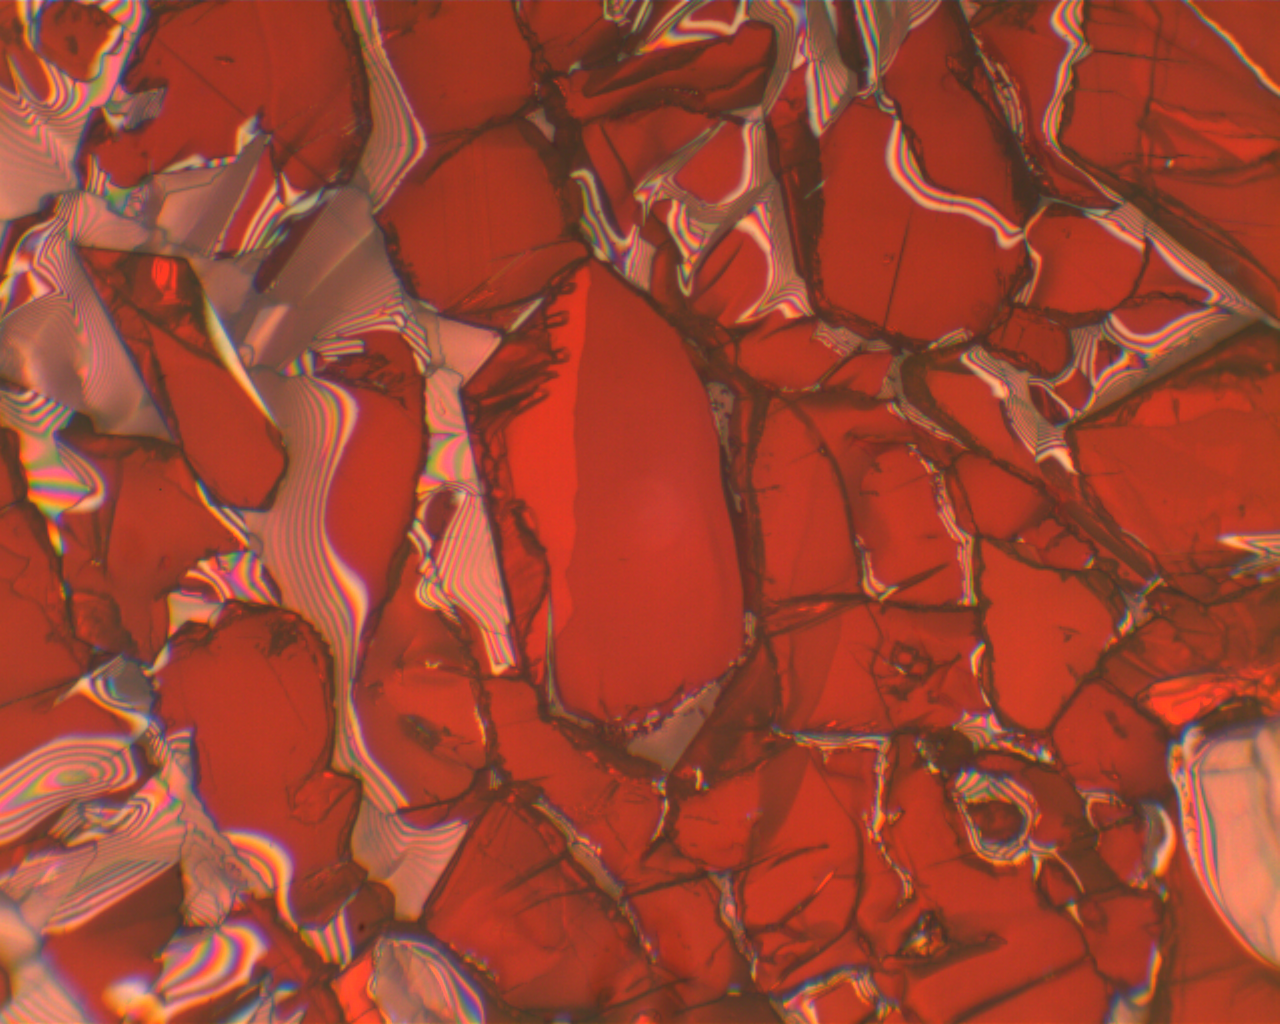
\includegraphics[width=\textwidth]{./img/tesf-white-illum.png}
        % \caption{TESF region of interest under white light.}
        \caption{}
        \label{img:tesf-white}
    \end{subfigure}
    \hfill
    \begin{subfigure}[b]{0.45\textwidth}
        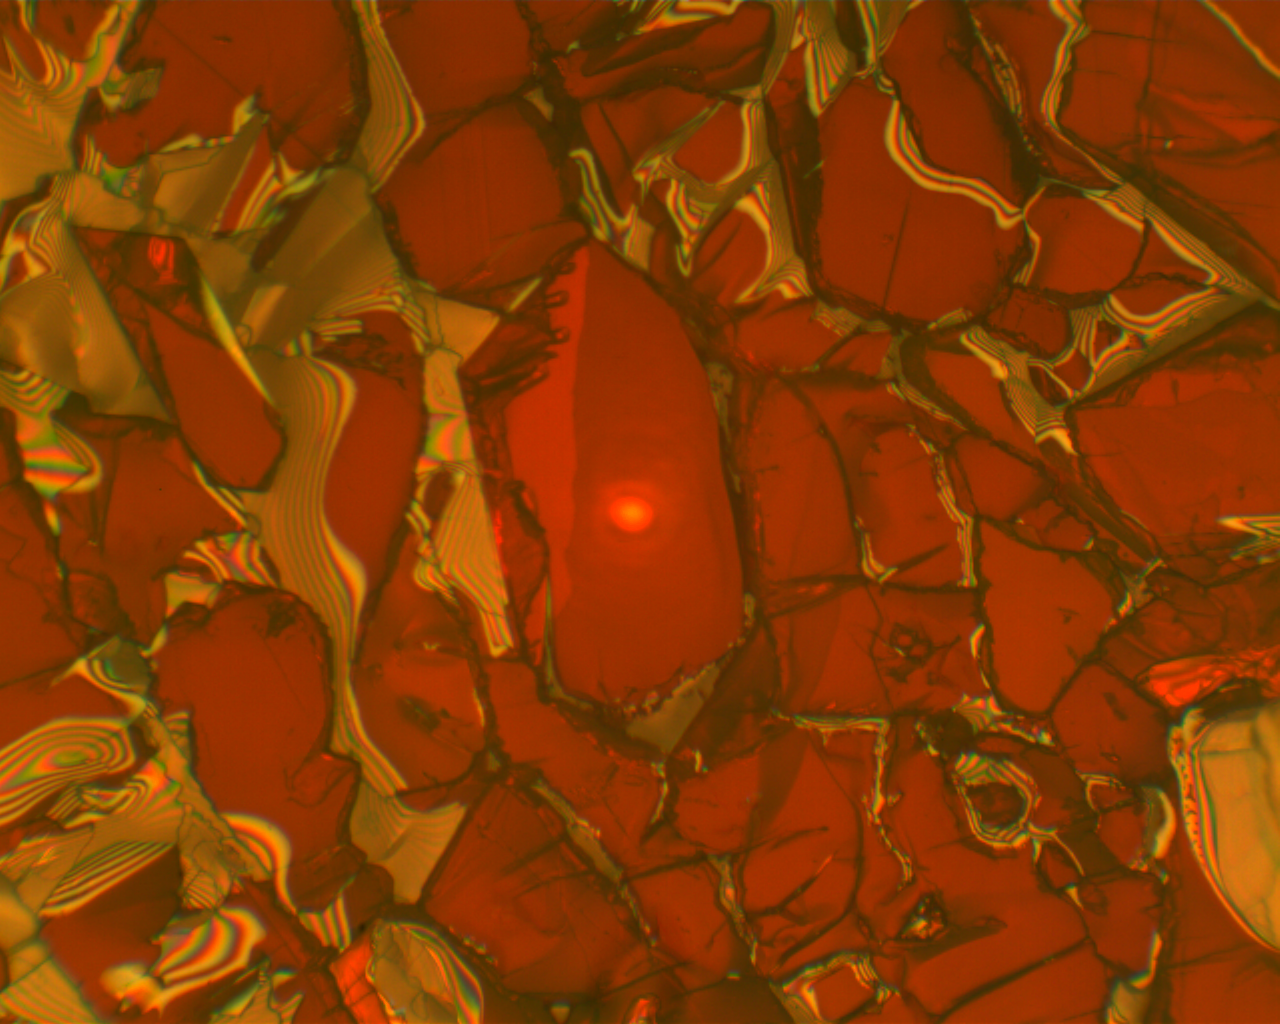
\includegraphics[width=\textwidth]{./img/tesf-laser-illum.png}
        % \caption{TESF region of interest under excitation light.}
        \caption{}
        \label{img:tesf-laser}
    \end{subfigure}
    \caption[Images of ADT TES-F sample.]{Images of ADT TES-F sample under white light (\ref{img:tesf-white}) and under laser excitation light (\ref{img:tesf-laser}). Reflected excitation light was optically filtered out of Figure \ref{img:tesf-laser} using a dichroic mirror and colored glass longpass filter. Photoluminescence spectra of this region are shown in Figure \ref{fig:pl-adt-tesf}.}
    \label{img:tesf}
\end{figure}

\begin{figure}[H]
    \centering
    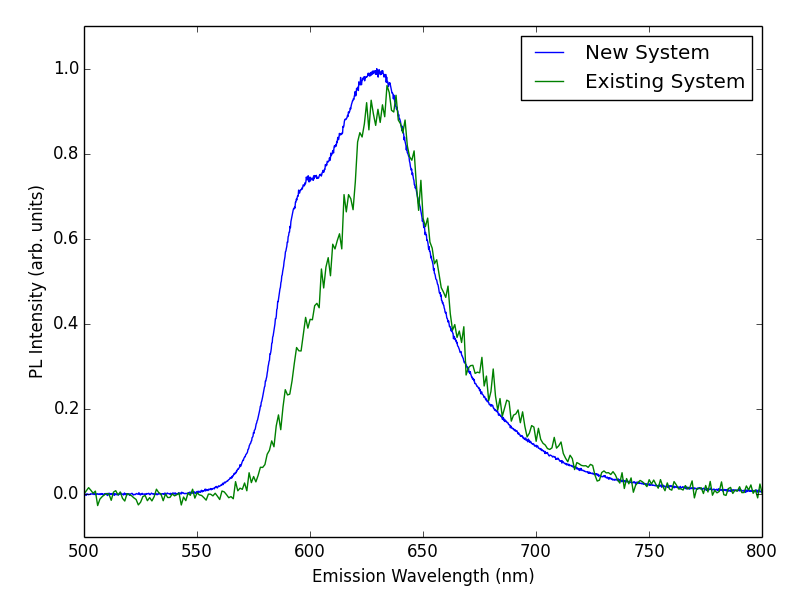
\includegraphics[width=0.8\textwidth]{./img/tesf-2.png}%\llap{\raisebox{4cm}{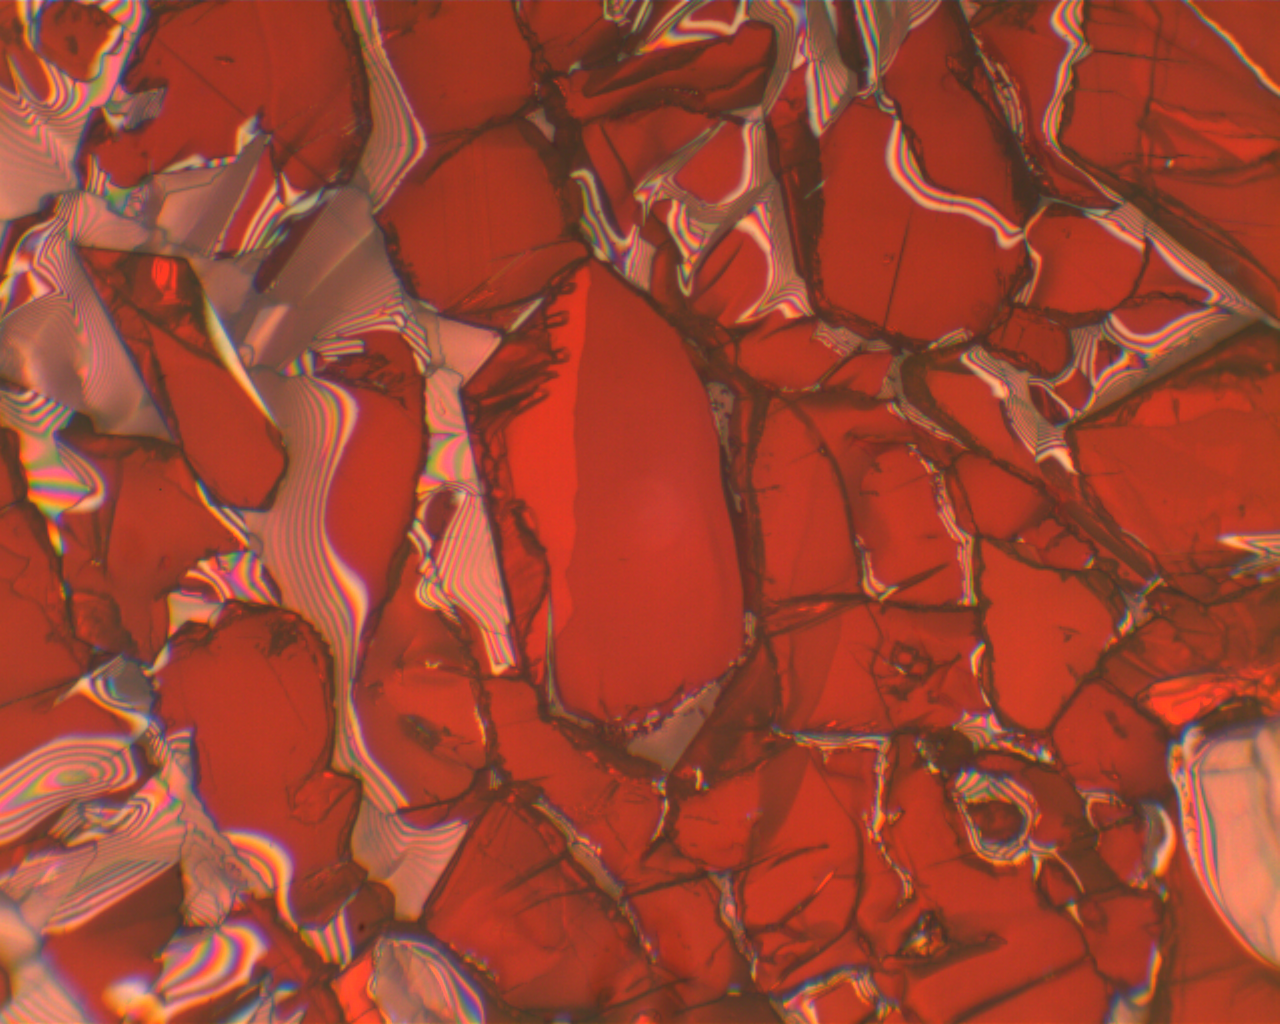
\includegraphics[width=2cm]{img/tesf-white-illum.png}}}
    % 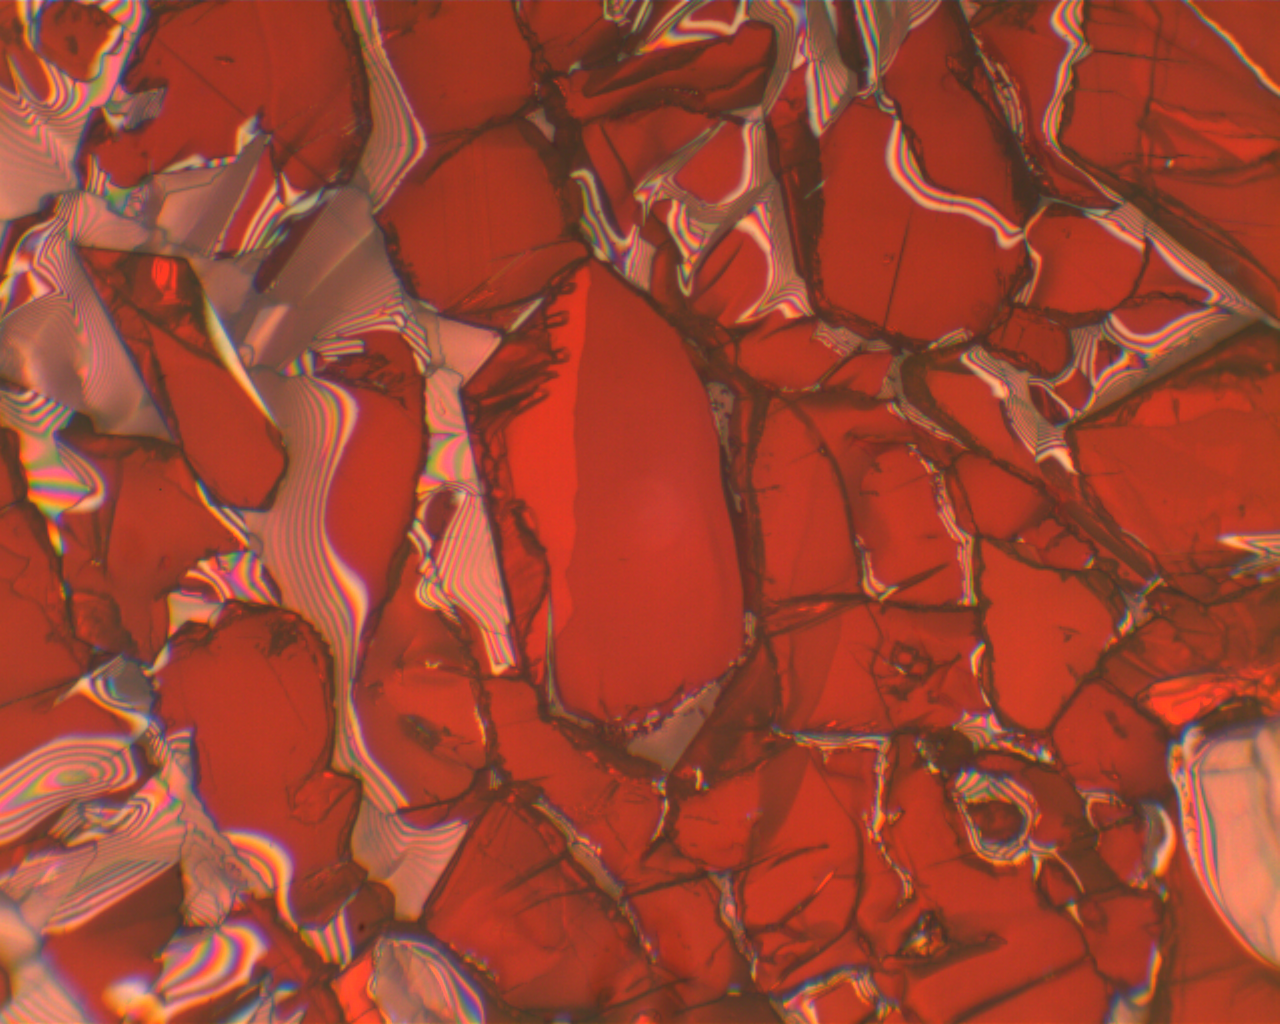
\includegraphics[width=.2\textwidth]{./img/tesf-white-illum.png}
    % 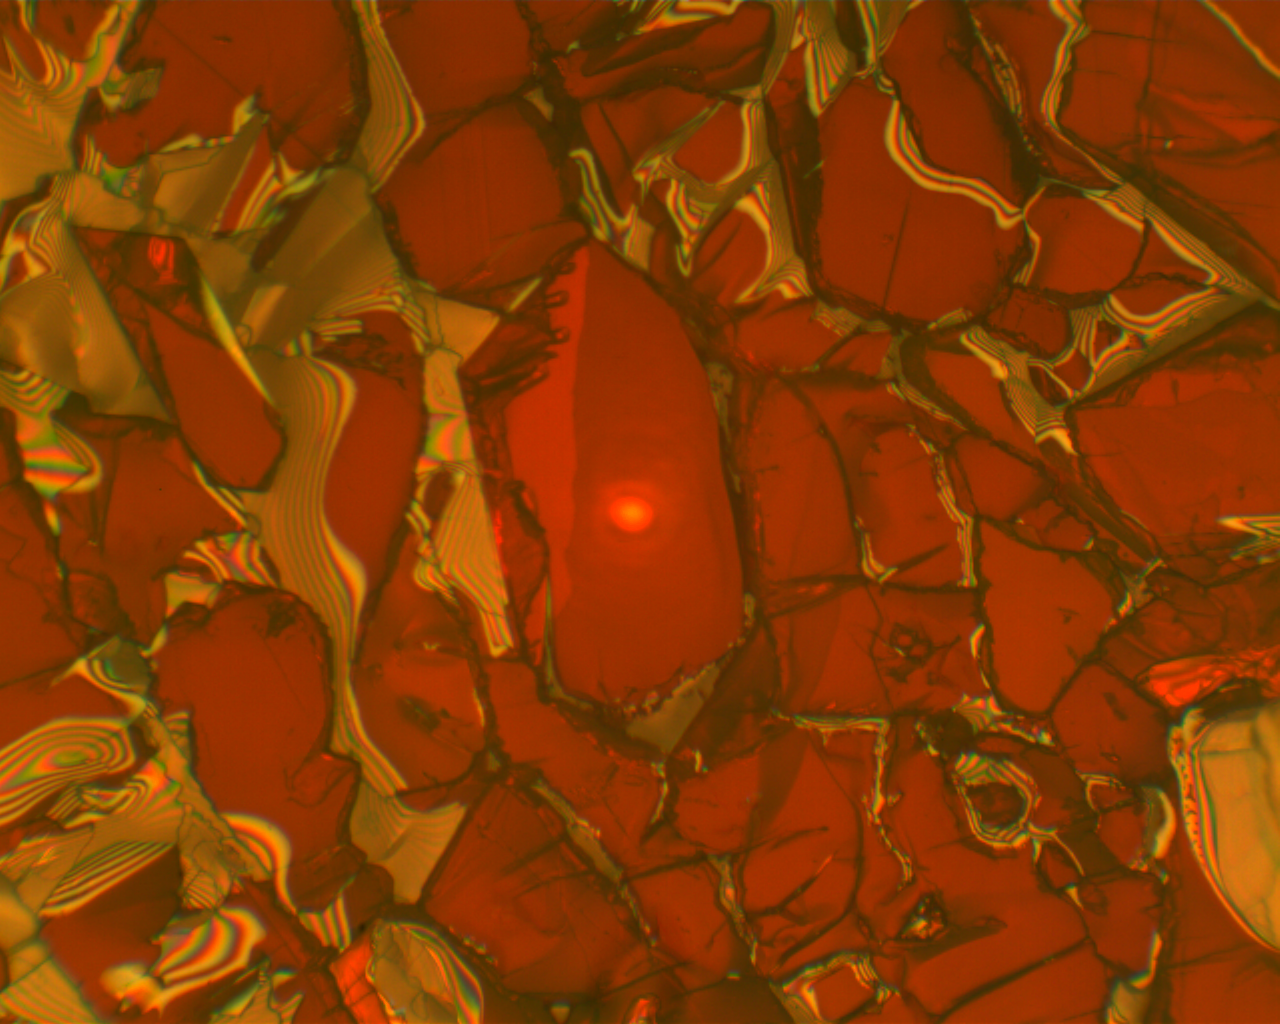
\includegraphics[width=.2\textwidth]{./img/tesf-laser-illum.png}
    \caption[PL emission spectrum of ADT TES-F, excited at 405nm.]{PL emission spectrum of ADT TES-F, excited at 405 nm.}
    \label{fig:pl-adt-tesf}
\end{figure}

The results from the microspectrometer show an emission maximum at 630 nm for the ADT TES-F sample; a less intense local maximum is also shown at about 600 nm. The spectrum measured with the Fluorolog has similar features to that of the microspectrometer, but is not precisely the same. The peak appears narrower overall in the Fluorolog data than in the microspectrometer data. The lower-wavelength side of the peak begins to rise at a higher wavelength in the Fluorolog data, and the emission maximum is red-shifted by about 4 nm. The local maximum at 600 nm is much less prominent in the Fluorolog data than in the microspectrometer data.

The microspectrometer data shows emission peaks similar to the ones reported by Shepherd \emph{et al.}, who used a similar drop cast sample and the same model Ocean Optics spectrometer \cite{e._b._shepherd_effect_2011}. Unlike Shepherd, we were not able to calibrate our detector with a reliable instrument; this could be a cause for the slight shift between peaks in the Fluorolog data as compared to our microspectrometer data.

Crystal aggregates and orientation with respect to the polarization of the excitation light have been shown to affect the emission spectra in ADT derivatives \cite{lam_polarization_2018}. As shown in Figure \ref{img:tesf}, we were able to excite what appears to be a single crystal domain --- assuming that this domain has few defects and a relatively uniform stacking structure, we expect it to fluoresce with a distinct spectrum. The Fluorolog excites a much wider area of the sample, which may include many crystal domains, defects, and slightly different stacking structures. Thus, it is conceivable that the resulting fluorescence spectrum is an aggregate of several slightly different spectra.

\begin{figure}[H]
    \centering
    \begin{subfigure}[b]{0.45\textwidth}
        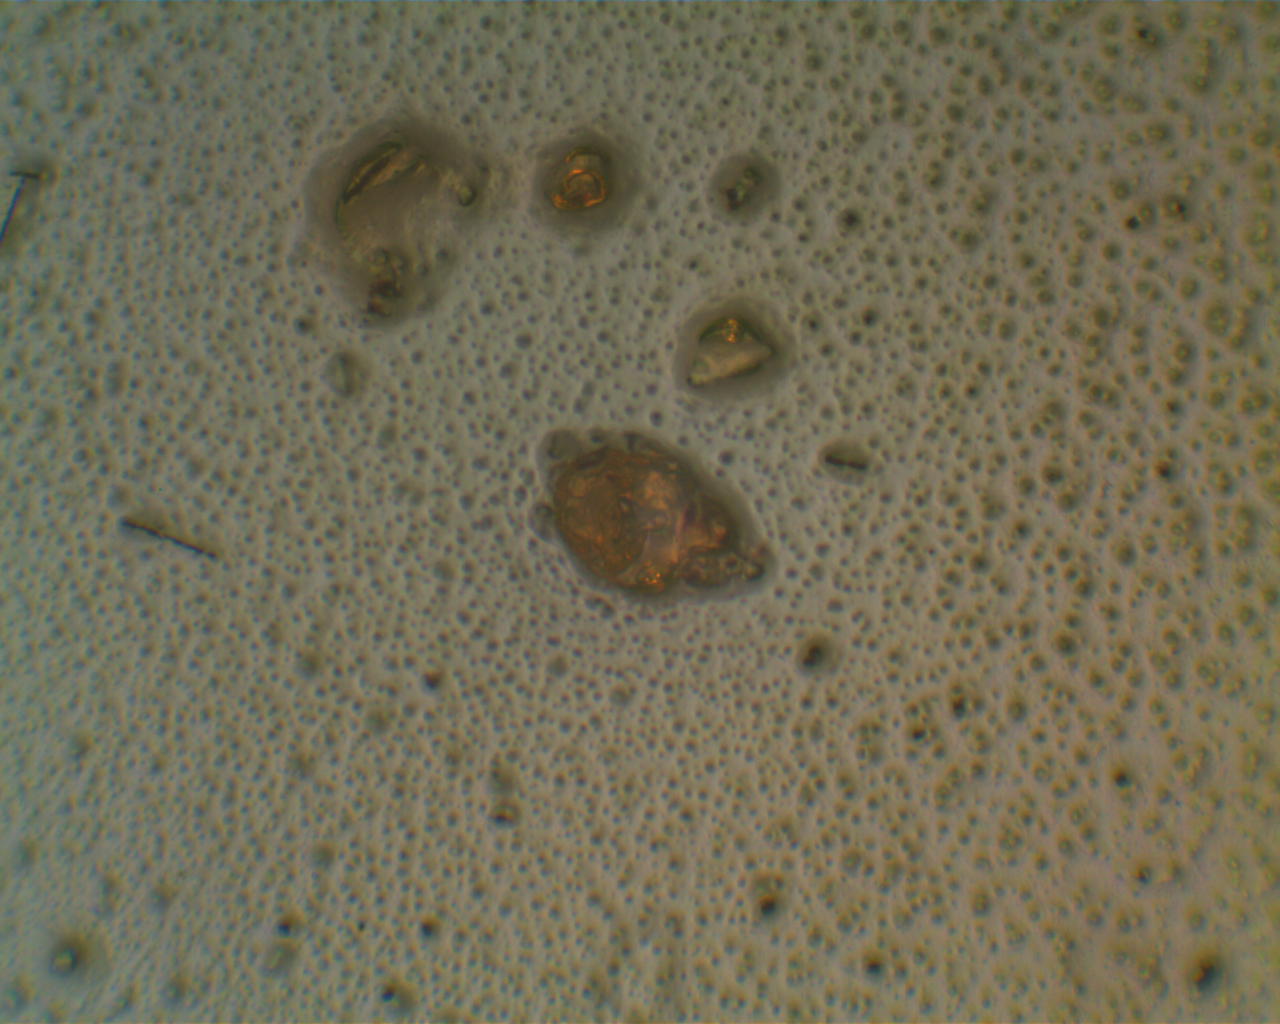
\includegraphics[width=\textwidth]{./img/qd-white-illum.png}
        \caption{}
        \label{img:qd-white}
    \end{subfigure}
    \hfill
    \begin{subfigure}[b]{0.45\textwidth}
        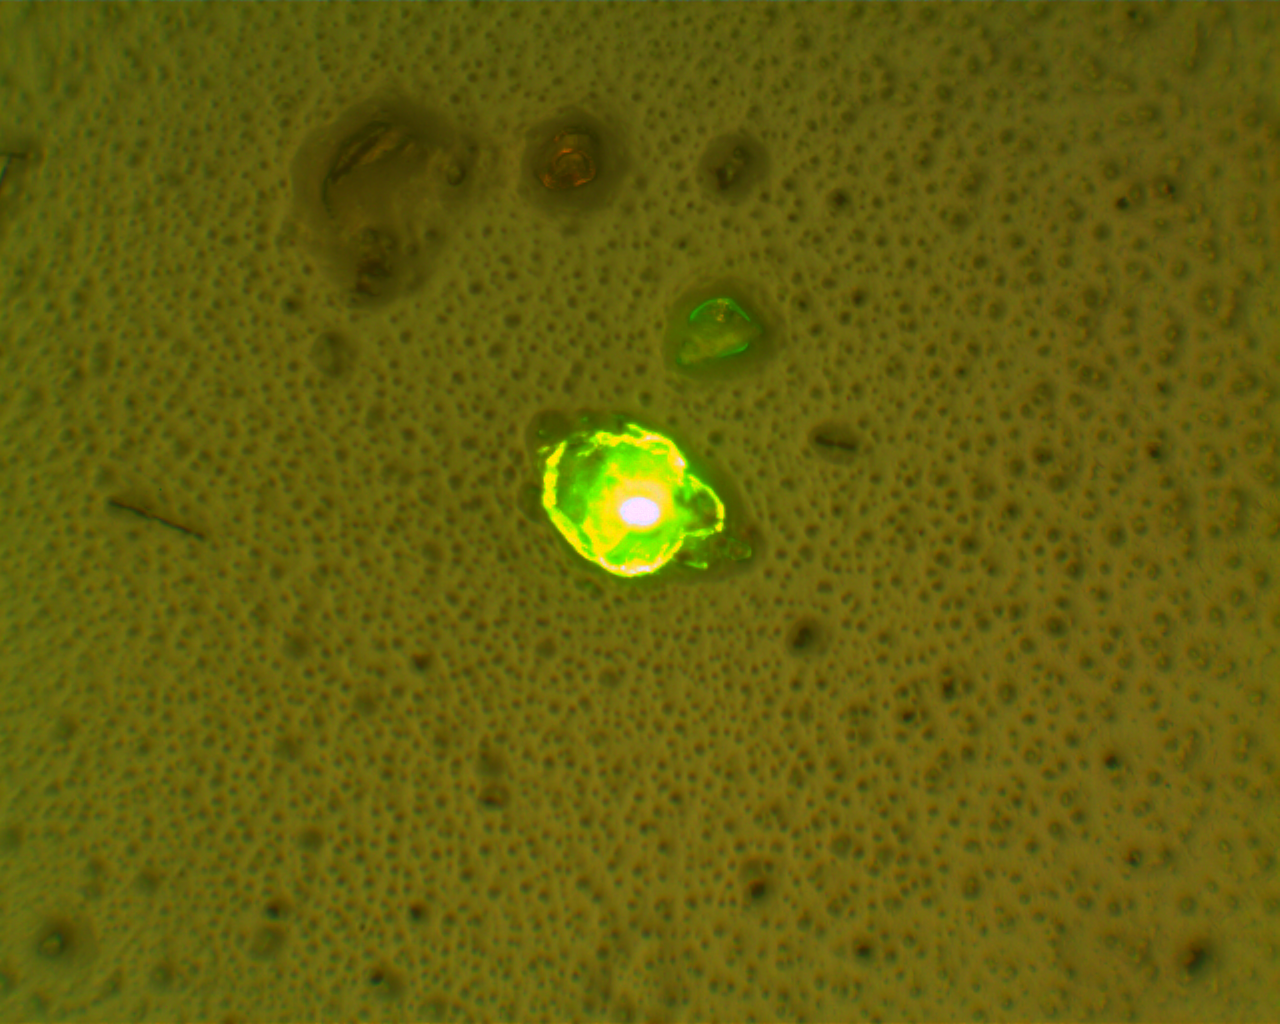
\includegraphics[width=\textwidth]{./img/qd-laser-illum.png}
        \caption{}
        \label{img:qd-laser}
    \end{subfigure}
    \caption[Images of CdSe quantum dot sample.]{Images of CdSe quantum dot sample under white light (\ref{img:qd-white}) and under laser excitation light (\ref{img:qd-laser}). Reflected excitation light was optically filtered out of Figure \ref{img:qd-laser} with a dichroic mirror and colored glass longpass filter. Photoluminescence spectra of this sample are shown in Figure \ref{fig:pl-adt-qd}.}
    \label{img:qd}
\end{figure}

\begin{figure}[H]
    \centering
    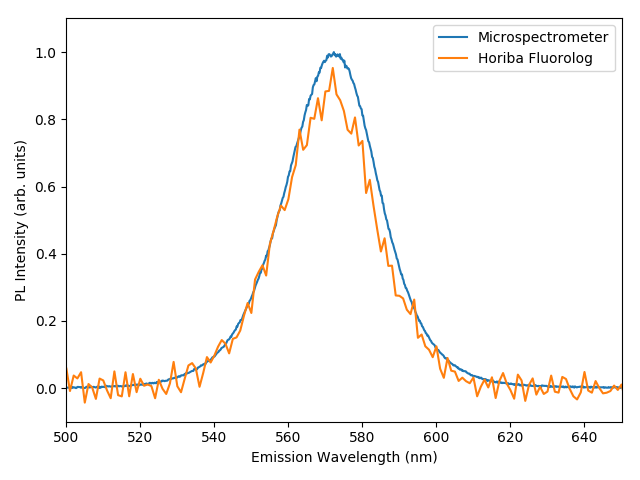
\includegraphics[width=0.8\textwidth]{./img/qd-2.png}
    % 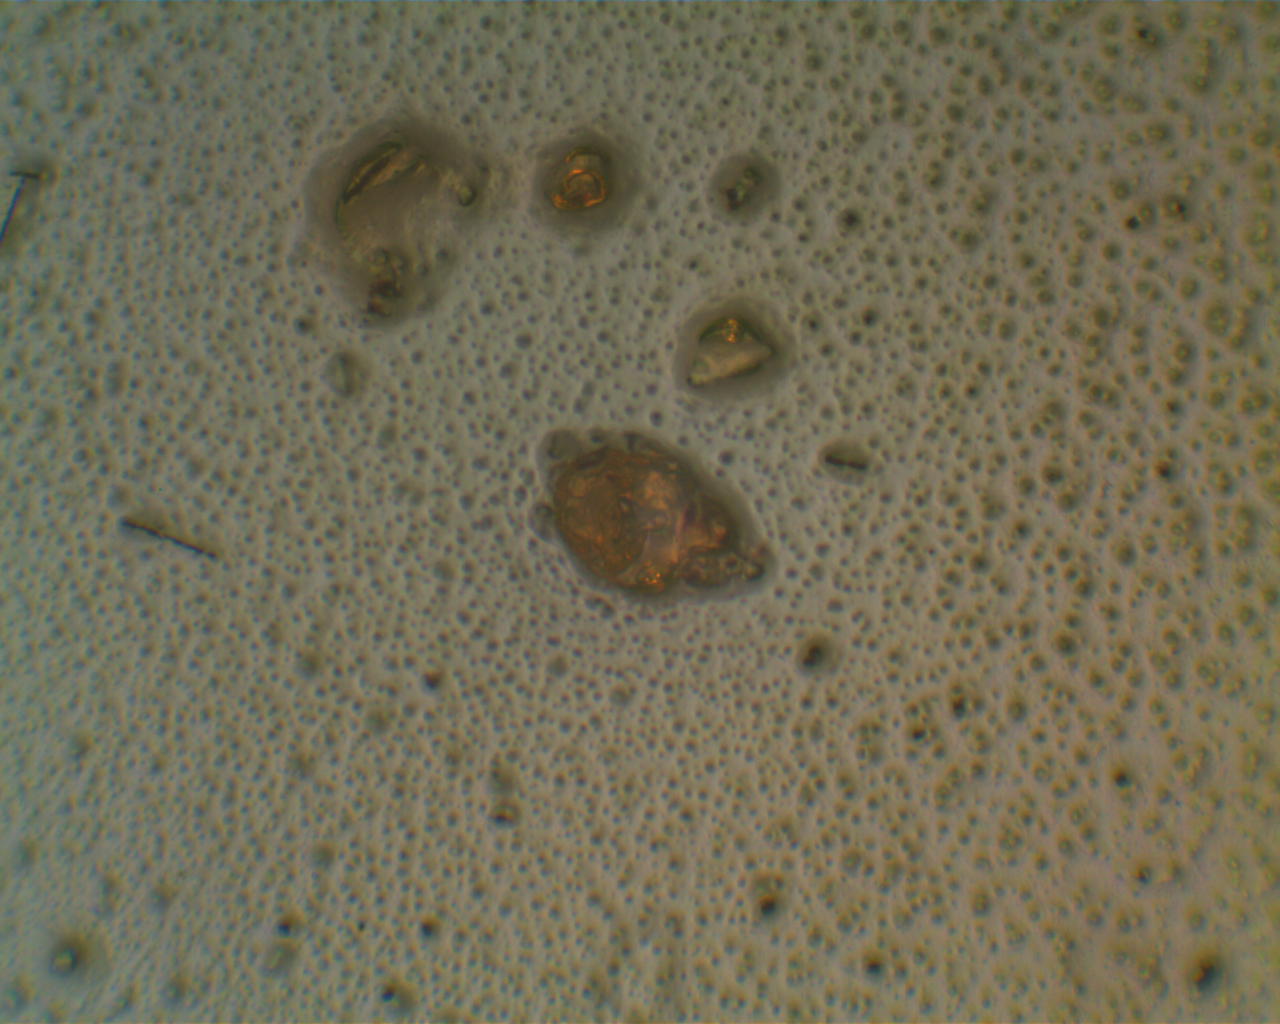
\includegraphics[width=4cm]{./img/qd-white-illum.png}
    % 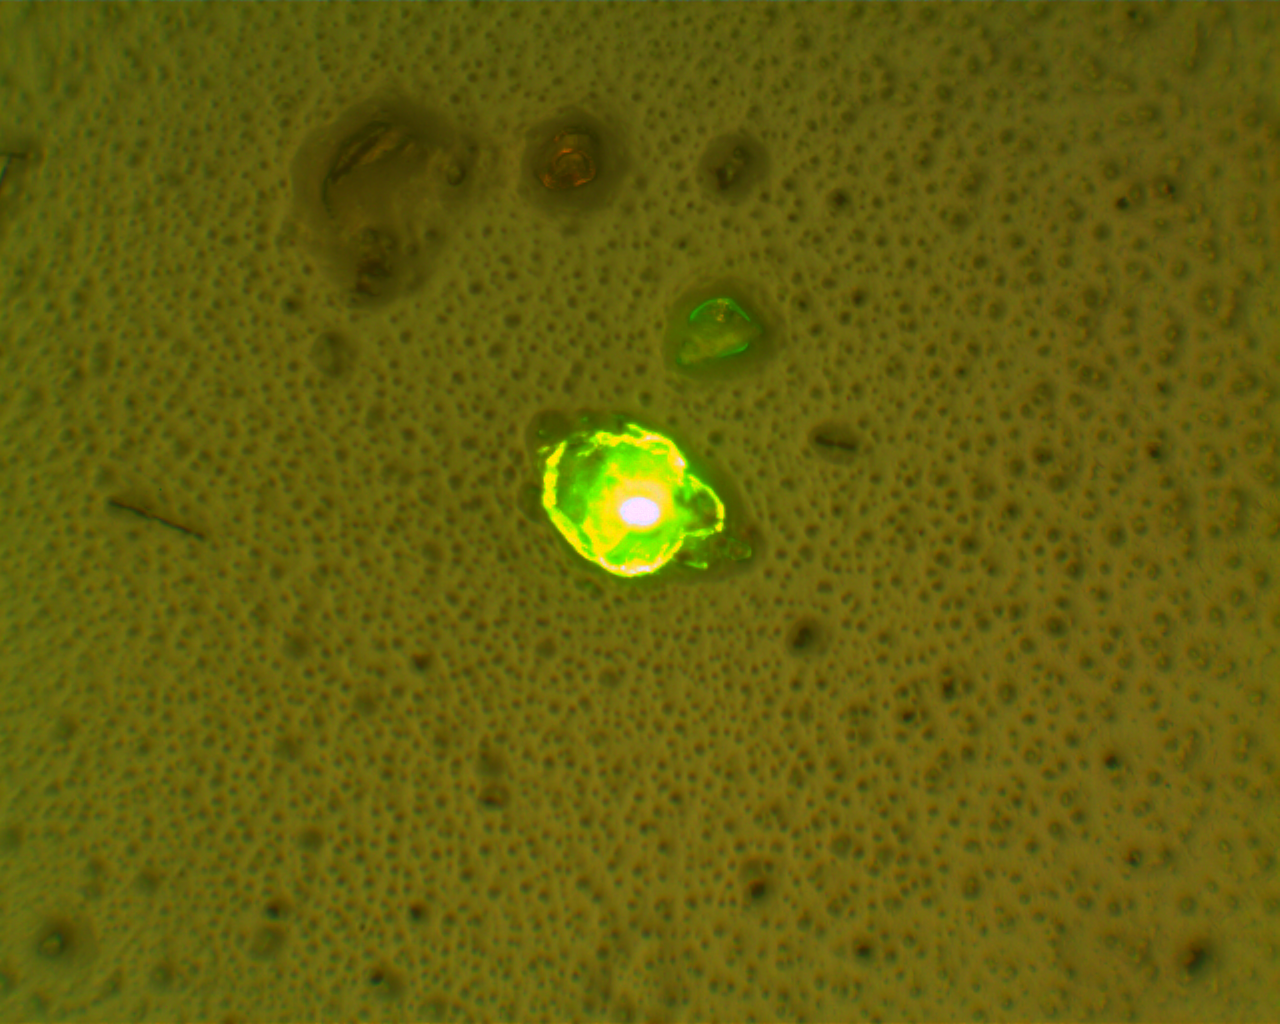
\includegraphics[width=4cm]{./img/qd-laser-illum.png}
    \caption{PL emission spectrum of a cluster of CdSe quantum dots, excited at 405 nm.}
    \label{fig:pl-adt-qd}
\end{figure}

The microspectrometer data shows an emission maximum at 572 nm for our sample of CdSe quantum dots. Peaks in both the Fluorolog and microspectrometer data are well-aligned, though there is a very slight blue-shift in the higher-wavelength leg of the peak of the Fluorolog data. 

The peak at 572 nm is also reported by Empedocles \emph{et al.} in their paper, "Photoluminescence Spectroscopy of Single CdSe Nanocrystallite Quantum Dots" \cite{empedocles_photoluminescence_1996}. They report a much narrower peak than we found (13 meV FWHM to our 110 meV), but measure PL at a very high excitation intensity. We are unable to thoroughly compare our results to those published by Empedocles because we do not have excitation intensity data, but it is possible that excitation intensity affected the width of our emission peak. It is also possible that fundamental differences in our sample and methods resulted in a wider peak --- it is well known that fluorescence in quantum dots varies with their shape and size, and Empedocles used techniques beyond the scope of this project to measure PL of single quantum dots.

Data from the Fluorolog is notably more noisy than data from our microspectrometer. It is possible that this is the result of smoothing by the Ocean Optics spectrometer and its software, though we have found no evidence to support this. It has been suggested that low excitation intensity when using the Fluorolog may result in noisy data, but we are unable to verify this because we do not have excitation intensity data for either of the instruments used in this work \cite{minot-private}. Future work with our microspectrometer instrument should make optical power measurements a high priority.
